\section{Problem analysis}
\ninanotes{
\begin{itemize}
\item Coarse problem analysis Describing the problem and goals in more
detail, briefly analysing the challenges, pointing out possible solutions.
\item Problem specification and analysis Detailed specification of the
problem (and goals). This might need to introduce new notation in order
to arrive at a precise description. If relevant, make state-of-the-art
solutions precise and compare.
\item Goals and success criteria Describe the goals and when a goal is
reached.
\end{itemize}
}

\subsection{Hardware and time constraints}
In order to run the self-play of the agents I will have to pick a platform to work on.
The setup I am gonna run the self-play of the agents on is utilizes an Intel® Core™ i7-10875H Processor, with 8 cores and 16 GB of ram. There are also 34GB of swap memory. So there are about 50 GB of memory as an constraint.
In regards to time constraint I want to make have that each agent does not spent much more time than a real-time player. A couple of minutes at most - but this goal is less important, but mostly there to secure that it is actually testable.
The chosen setup and time and memory constraints is mainly due to that is the computer I got, and I now I can iterate fast over a setup I have full control over.

% Inspired by the multi-modal logic \KTfourfiveN


\subsubsection{Three wise men puzzle}
In order to motivate my approach to the problem, namely multi-modal logic. 
I will take the example of the three wise men problem.
There are three wise men, each standing in a row, enumarated 1 through 3. 
Then a king, who has 3 red hats and 2 white hats puts a hat on each of the three wise men in such a way that each person does not know which hat he put on their head. 
Then the king asks the first wise man whether he knows the color of their own hat, where the answers could either be "I don't know" or "I know". 
He then asks the same of the second, then the third.

Let us say that the actual case is RRR i.e. wise man 1, 2 and 3 has a red hat on their head.
In that case wise man 1 will answer: I don't know, the second wise man will answer: I don't know, but the third wise man will answer: I know, how so?

Trying to see the problem from the third wise man's perspective we have the following model. It is based on \KTfourfiveN in \cite{HuthAndRyan2004}, but breaks with convention used by them in the following way:
The model is strictly from the perspective of wise man 3. So for each possible world of wise man 3, we "fix" this world and then imagine what the other wise men could think was possible based on this. An edge with label x means that wise man x knows this is possible, based on the fixed world of wise man 3.
\begin{figure}[H]
	\center
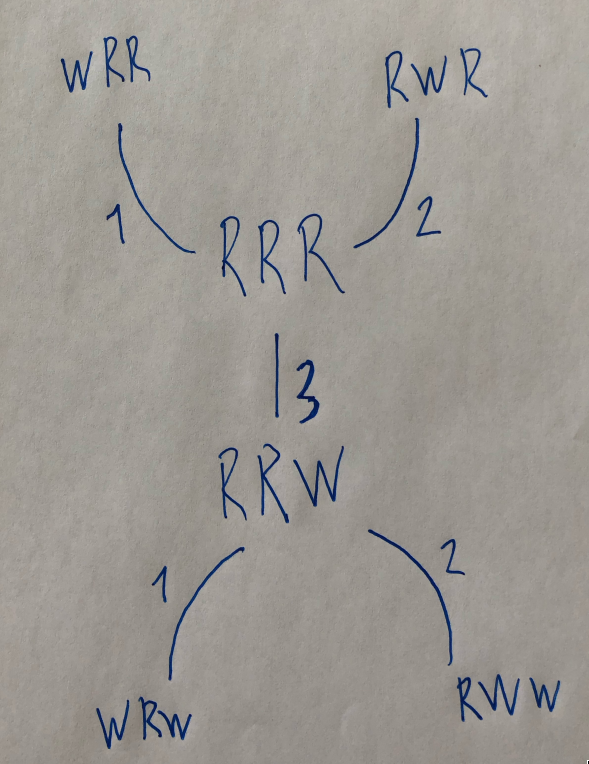
\includegraphics[width=10cm]{images/three_wise_men_round_0.png}
\end{figure}
This is initial configuration meaning, wise man three does not know whether he has a red hat or a white hat. And for each of these fixed scenarios he can imagine that 2 cannot know either, and neither can 1.

But when 1 states "he does not know" then that has to be equivalent to "not RWW is the case". This means that three can safely eliminate this state, as something 2 would imagine, given that this was a public announcement. This results in this state:
\begin{figure}[H]
	\center
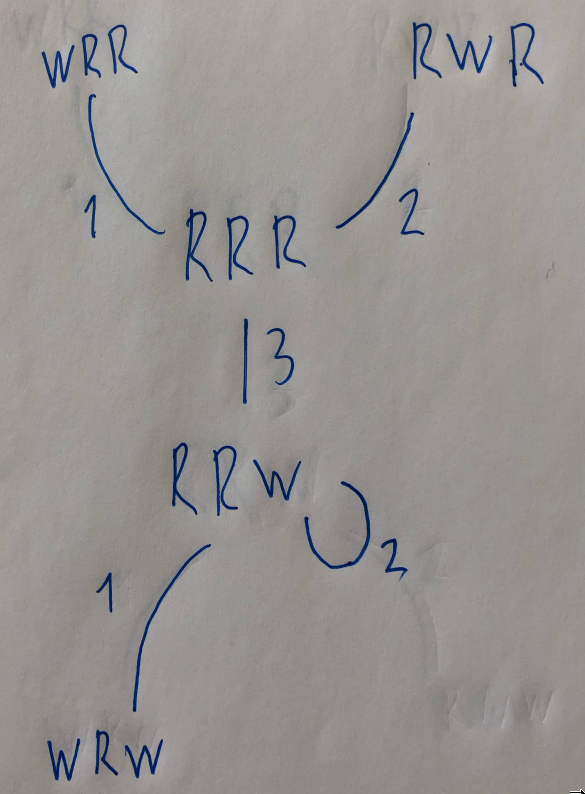
\includegraphics[width=10cm]{images/three_wise_men_round_1.png}
\end{figure}

After 2 answers "I don't know", wise man 3 can deduce that the case was not RRW. Which means that the final structure is:

\begin{figure}[H]
	\center
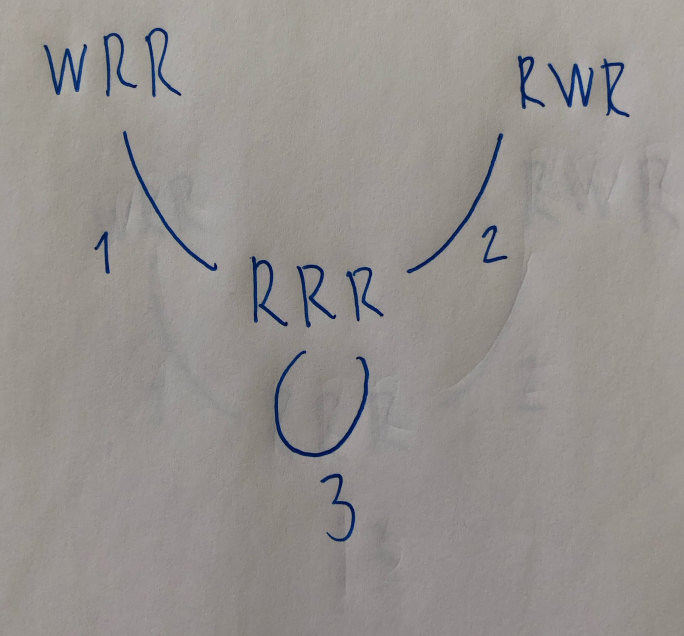
\includegraphics[width=10cm]{images/three_wise_men_round_2.png}
\end{figure}

These concepts can be ported to Hanabi quite analogously






\subsection{Problems with possible worlds and modal logic}
The problem with making cooperative agents in hanabi - especially when you want to use modal logic - is mainly due to the fact that each agent does not know its own hand, and this lack of knowledge leads to a huge number of possible worlds. 
A naive approach to represent this lack of knowledge is simply to generate all possible hands given the information the agent has.
This, I would argue, is pretty straight-forward to work with, but if done in a bad way will lead to intolerable waiting times and/or memory usage.

For example let us denote a game played by two players Alice and Bob. 

\todo[inline]{Make notation for the entire set (i.e. the kripkestructure) and just for the set of hands from a players perspective}
If Alice sees Bobs cards (and the discard pile, and hanabi pile), then Alice can generate the set of possible hands $\mathcal{H}$.
But in order to also represent the knowledge of Bob, Alice would have to for each $h \in \mathcal{H}$ generate a new set of possible hands for Bob $H_{Bob}$, which for each $h$ would be the set of hands Bob considers possible from the information he lacks and the world $h$ Alice assumes to be true. 
This seems to be the approach taken by \cite{EgerM17}.
To optimize this approach, one could store the hints and shown cards at the agents, and at some proper time -- when a significant amount of hints and cards have been revealed -- produce the set $\mathcal{H}$ and the relevant sets for the other players.

Trying to quantify the number of possible hands for a single agent I have simulated 30 random games and come up with this table

\begin{table}[]
\begin{tabular}{l|llll}
Number of players & 2       & 3       & 4       & 5      \\
Mean              & 83369.9 & 64134.8 & 11696.5 & 9190.4 \\
Median            & 82956.5 & 61055.0 & 11759.0 & 8926.5 \\
Min               & 65574   & 47666   & 7406    & 6676   \\
Max               & 93667   & 83848   & 16316   & 12962 
\end{tabular}
	\caption{Simulated 30 games, dealt the cards to all the players except for 1 player, and calculated how many distinct combinations she could get (see how data is generated by Appendix \ref{appendix:python-distinct-combinations}).}
\end{table}


Looking at the different setups, there are a huge number of combinations for the 2 player setup. If we assume

